\documentclass[english,handout]{mlutalk}

\title{%
  Modern Talking: Key-Point Analysis \\
  using Modern Language Understanding
}
\subtitle{Natural Language Processing, Summer Semester 2021}
\author{Max Henze \and Hanh Luu \and Jan Heinrich Reimer}
\institute{Martin Luther University Halle-Wittenberg}
\date{June 29, 2021}
\titlegraphic{
\includegraphics[width=3cm]{figures/mlu-halle}}

\addbibresource{../literature/literature.bib}

\usepackage{tikz}
\usetikzlibrary{positioning}
\usepackage{listings}
\usepackage{xspace}
\usepackage{biblatex}
\usepackage{tabularx}
\usepackage{booktabs}
\usepackage{graphics,graphicx}

\newcommand{\Bert}{\textsc{Bert}\xspace}
\newcommand{\ArgKP}{\mbox{ArgKP}\xspace}
\newcommand{\ArgQ}{\mbox{IBM-ArgQ-Rank-30kArgs}\xspace}
\newcommand{\BiLSTM}{\mbox{BiLSTM}\xspace}
\newcommand{\BertBase}{\textsc{Bert}-Base\xspace}
\newcommand{\BertLarge}{\textsc{Bert}-Large\xspace}
\newcommand{\TF}{\mbox{TF}\xspace}
\newcommand{\TFIDF}{\mbox{TF/IDF}\xspace}
\newcommand{\todocite}{{\smaller\color{red}[CITE]}\xspace}
\newcommand{\todo}[1]{{\smaller\color{red}[#1]}}

\tikzset{%
    every neuron/.style={
      circle,
      draw,
      minimum size=1cm
    },
    neuron missing/.style={
      draw=none, 
      scale=4,
      text height=0.333cm,
      execute at begin node=\color{black}$\vdots$
    },
    layer/.style= {
      rectangle,
      draw,
      minimum size = 1cm
    }
  }

\begin{document}

\titleframe

\begin{frame}{Initial Ideas}
  
  \begin{itemize}
    \item Rule-based baseline
    \item Improve upon the baseline with Machine Learning
    \begin{itemize}
      \item Regression, SVC~\todocite
      \item Ensemble
      \item Deep Neural Networks, e.g., \BiLSTM~\todocite with GloVe embeddings~\todocite, \Bert~\todocite
    \end{itemize}
    \item Variations of the above \(\to\) Hyper-parameter tuning
  \end{itemize}
  
  \begin{block}{What did not work?}
    Some of the brainstormed ideas did not improve upon the baseline:
    \begin{itemize}
      \item Regression, SVC
      \item Ensemble
      \item \BiLSTM
    \end{itemize}
  \end{block}

\end{frame}

\begin{frame}{Regression, SVC}
  
  \framesubtitle{What did not work?}
  
  \begin{itemize}
    \item Features: bag-of-words and/or \TFIDF for selected parts-of-speech
    \item Regression \todo{what type?}, Support Vector Classifier
    \item Ensemble of Regression + SVC
  \end{itemize}
  
  \begin{block}{Technology}
      \begin{itemize}
        \item NTLK~\todocite for tokenization \todo{didn't we?}, stemming,  and stop word list
        \item spaCy~\todocite for part-of-speech tagging
        \item Scikit-Learn~\todocite for bag-of-words and \TFIDF
        \item Scikit-Learn~\todocite for regression and SVC implementation
      \end{itemize}
  \end{block}

\end{frame}

\begin{frame}{Regression, SVC}

  \framesubtitle{Why did not work?}

  \begin{itemize}
    \item Too much features~(\( > 4000 \)) for Regression
    \item SVC better results, but still worse than baseline
    \item Can't capture context or semantic meaning
  \end{itemize}

  \begin{example}[False Positives]
    \smaller
    \begin{tabular}{ll}
      Argument: & School uniforms violate the right to freedom of expression. \\
      Key Point: & School uniforms are often uncomfortable/sexist. \\
      Prediction: & Match
    \end{tabular}
  \end{example}
  
  \begin{example}[False Negatives]
    \smaller
    \begin{tabular}{ll}
      Argument: & It is not fair to not allow children to express their personality through dress as long as it is appropriate. \\
      Key Point: & School uniform is harming the student's self expression. \\
      Prediction: & No match
    \end{tabular}
  \end{example}

\end{frame}

\begin{frame}[allowframebreaks]{Term Overlap}
  
  \begin{itemize}
    \item Rule-based approach with no training
    \item Features: (preprocessed) terms
    \item Preprocessing:
    \begin{itemize}
      \item Stemming \(\leadsto\) generalization
      \item Stop words \(\leadsto\) less noise/confusion \\ modified without \query{not}
      \item Synonyms, antonyms \(\leadsto\) generalization
    \end{itemize}
    \item Compute similarity based on Jaccard similarity coefficient~\todocite, i.e., proportion of terms that appear in argument and key point
    \item Good improvement with preprocessing: up to 12~pp \todo{don't abbreviate}
  \end{itemize}
  
  \begin{example}[Preprocessing]
    \smaller
    Homeschooling a child denies them valuable lifeskills, particularly interaction with their own age group and all experiences stemming from this. \\
    \(\to\) homeschool child deni valuabl lifeskil particular interact age group experi stem
  \end{example}

  \framebreak
  
  \begin{block}{Technology}
      \begin{itemize}
        \item NTLK~\todocite for tokenization, stemming,  and stop word list
        \item WordNet~\todocite (via NLTK) for synonyms and antonyms
      \end{itemize}
  \end{block}

  \begin{block}{Intuition}
    \begin{itemize}
      \item Many arguments contain the same words as matching key points
      \item Key points summarize arguments
      \item Stemming/synonyms/antonyms increase overlap
    \end{itemize}

    \begin{example}
      \smaller
      \begin{tabular}{lp{0.7\textwidth}}
        Argument: & People reach their limit when it comes to their quality of life and should be able to end their {\color{blue} suffering}. This can be done with little or no {\color{blue} suffering} by {\color{orange} assistance} and the person is able to say good bye. \\
        Key Point: & {\color{orange} Assisted} suicide reduces {\color{blue} suffering}.
      \end{tabular}
    \end{example}
  \end{block}

\end{frame}

\begin{frame}{BiLSTM}
  \framesubtitle{Used technologies + Preprocessing}

  \begin{itemize}
    \item Tensorflow with Keras brings all RNN Technology
    \item NLPAUG for Augmenting Words
    
    \item Created different metrics how to deal with unlabeled pairs
      \begin{itemize}
        \item \textbf{skip} : use labeled pairs only
        \item \textbf{strict} : missing labels are seen as: "No Match"
        \item \textbf{relaxed} : missing labels are seen as: "Match"
      \end{itemize}
  \end{itemize}

  

\end{frame}


% \begin{frame}
%   \frametitle{BiLSTM}
%   \framesubtitle{}
%     %TODO cite paper which inspired to use blstm
%   \begin{figure}
%     \begin{tikzpicture}[x=1.5cm, y=1.5cm, >=stealth, scale = 1]
%       \node [every neuron] (arg) at (0,2.5) {arg};
%       \node [every neuron] (kp) at (0,1.5) {kp};
  
%       \node [layer] (wp) at (1.5, 2) {Word Piece};
%       \node [layer] (be) at (3.5, 2) {BERT Embedding};
  
%       \node [layer] (bm1) at (5.5, 3.5) {BiLSTM};
%       \node [layer] (bm2) at (5.5, 0.5) {BiLSTM};
  
%       \node [layer] (con) at (5.5, 2) {+};
%       \node [layer] (den) at (7, 2) {Dense};

%       \node [] (des) at (1.3,3.9) {\small BERT + BiLSTM};
  
%       \draw [->] (arg) -- (wp);
%       \draw [->] (kp) -- (wp);

%       \draw [->] (wp.20) -- (be.166);
%       \draw [->] (wp.340) -- (be.194);

%       \draw [->] (be.15) -- (bm1.180);
%       \draw [->] (be.345) -- (bm2.180);

%       \draw [->] (bm1.270) -- (con.90);
%       \draw [->] (bm2.90) -- (con.270);

%       \draw [->] (con) -- (den);

%       \draw [->] (den) -- (7.8 ,2);

%       \draw[draw=red] (7.5,0) rectangle (0.5,4);
%     \end{tikzpicture}
%   \end{figure}
% \end{frame}

\begin{frame}{BiLSTM}
  \framesubtitle{Approach}
    %TODO cite paper which inspired to use blstm
  \begin{figure}
    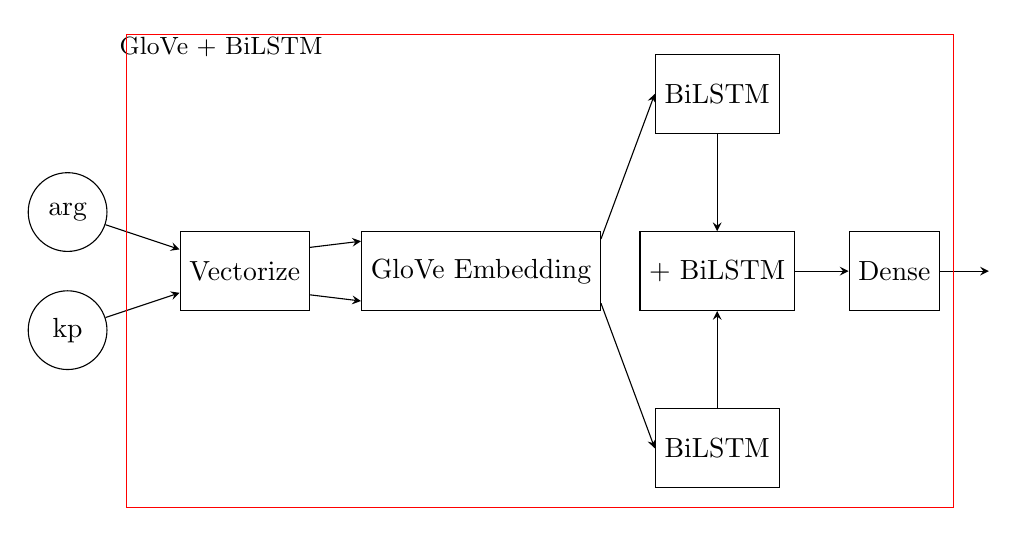
\begin{tikzpicture}[x=1.5cm, y=1.5cm, >=stealth, scale = 1]
      \node [every neuron] (arg) at (0,2.5) {arg};
      \node [every neuron] (kp) at (0,1.5) {kp};
  
      \node [layer] (wp) at (1.5, 2) {Vectorize};
      \node [layer] (be) at (3.5, 2) {GloVe Embedding};
  
      \node [layer] (bm1) at (5.5, 3.5) {BiLSTM};
      \node [layer] (bm2) at (5.5, 0.5) {BiLSTM};
  
      \node [layer] (con) at (5.5, 2) {+ BiLSTM};
      \node [layer] (den) at (7, 2) {Dense};

      \node [] (des) at (1.3,3.9) {\small GloVe + BiLSTM};
  
      \draw [->] (arg) -- (wp);
      \draw [->] (kp) -- (wp);

      \draw [->] (wp.20) -- (be.166);
      \draw [->] (wp.340) -- (be.194);

      \draw [->] (be.15) -- (bm1.180);
      \draw [->] (be.345) -- (bm2.180);

      \draw [->] (bm1.270) -- (con.90);
      \draw [->] (bm2.90) -- (con.270);

      \draw [->] (con) -- (den);

      \draw [->] (den) -- (7.8 ,2);

      \draw[draw=red] (7.5,0) rectangle (0.5,4);
    \end{tikzpicture}
  \end{figure}
\end{frame}

\begin{frame}{BiLSTM}
  \framesubtitle{Predictions on why did it not work ?}
    
  Tested a lot of different parameter settings:
  \begin{itemize}
    \item Epochs
    \begin{itemize}
      \item Few $(1-10)$ resulted in good scores on training set but mediocre on dev set
      \item A lot $(10-100)$ resulted in decreasing \texttt{val\_acc} $\rightarrow$ Overfiting
      \item Used EarlyStopping, Dropout and Weight Decay against it
    \end{itemize}
  \end{itemize}
  Maybe we were learning to quickly or our data was not enough:
  \begin{itemize}
    \item Learning Rate 
    \begin{itemize}
      \item Set to $0.0001$ showed no significant improvement
    \end{itemize}
    \item Text Augmentation
    \begin{itemize}
      \item Creating new data from old for better generalization
      \item Yielded no improvement
    \end{itemize}
  \end{itemize}

  At this point: model probably to difficult or wrong way of data input

\end{frame}

\begin{frame}{\Bert}
  \framesubtitle{Used technologies + Preprocessing}
  

\end{frame}

\begin{frame}{\Bert}
  \framesubtitle{Approach + Parameters}
  

\end{frame}

% EVALUATION OF BASELINE AND APPROACHES

\begin{frame}
  \frametitle{Evaluation}
  \begin{figure}
    \centering
    \scalebox{0.70}{
      \begin{tabular}{lrrrlrrr}
          \multicolumn{8}{c}{\textbf{\Large Mean Average Precision}}\\
          \hspace{1em}\\
        \toprule
          Baselines/Approach & \multicolumn{3}{c}{Training Data} & & \multicolumn{3}{c}{Validation Data}\\ \cline{2-4} \cline{6-8}
          & Strict & Relaxed & Average & & Strict & Relaxed & Average\\
        \midrule
          Match All                           & 00000 & 00000 & 00000 & & 00000 & 00000 & 00000\\
          Match None                          & 00000 & 00000 & 00000 & & 00000 & 00000 & 00000\\
          Term Overlap (no prepro)            & 00000 & 00000 & 00000 & & 00000 & 00000 & 00000\\
          Term Overlap (stem)                 & 00000 & 00000 & 00000 & & 00000 & 00000 & 00000\\
          Term Overlap (stem, stowo)          & 00000 & 00000 & 00000 & & 00000 & 00000 & 00000\\
          Term Overlap (stem, stowo, syn, ant)& 00000 & 00000 & 00000 & & 00000 & 00000 & 00000\\
        \midrule
          BiLSTM (GloVe embeddings)           & 00000 & 00000 & 00000 & & 00000 & 00000 & 00000\\
          BERT-Base (skip)                    & 00000 & 00000 & 00000 & & 00000 & 00000 & 00000\\
          BERT-Large (skip)                   & 00000 & 00000 & 00000 & & 00000 & 00000 & 00000\\
          RoBERTa-Base (skip)                 & 00000 & 00000 & 00000 & & 00000 & 00000 & 00000\\
          DistilBERT-Base (skip)              & 00000 & 00000 & 00000 & & 00000 & 00000 & 00000\\
          Transformers                        & 00000 & 00000 & 00000 & & 00000 & 00000 & 00000\\
        \bottomrule
      \end{tabular}
    }
  \end{figure}
\end{frame}

\begin{frame}
  \frametitle{Evaluation cont.}
  \begin{figure}
    \centering
    \scalebox{0.70}{
      \begin{tabular}{lrrrlrrr}
          \multicolumn{8}{c}{\textbf{\Large Precision}}\\
          \hspace{1em}\\
        \toprule
          Baselines/Approach & \multicolumn{3}{c}{Training Data} & & \multicolumn{3}{c}{Validation Data}\\ \cline{2-4} \cline{6-8}
          & Strict & Relaxed & Average & & Strict & Relaxed & Average\\
        \midrule
          Match All                           & 00000 & 00000 & 00000 & & 00000 & 00000 & 00000\\
          Match None                          & 00000 & 00000 & 00000 & & 00000 & 00000 & 00000\\
          Term Overlap (no prepro)            & 00000 & 00000 & 00000 & & 00000 & 00000 & 00000\\
          Term Overlap (stem)                 & 00000 & 00000 & 00000 & & 00000 & 00000 & 00000\\
          Term Overlap (stem, stowo)          & 00000 & 00000 & 00000 & & 00000 & 00000 & 00000\\
          Term Overlap (stem, stowo, syn, ant)& 00000 & 00000 & 00000 & & 00000 & 00000 & 00000\\
        \midrule
          BiLSTM (GloVe embeddings)           & 00000 & 00000 & 00000 & & 00000 & 00000 & 00000\\
          BERT-Base (skip)                    & 00000 & 00000 & 00000 & & 00000 & 00000 & 00000\\
          BERT-Large (skip)                   & 00000 & 00000 & 00000 & & 00000 & 00000 & 00000\\
          RoBERTa-Base (skip)                 & 00000 & 00000 & 00000 & & 00000 & 00000 & 00000\\
          DistilBERT-Base (skip)              & 00000 & 00000 & 00000 & & 00000 & 00000 & 00000\\
          Transformers                        & 00000 & 00000 & 00000 & & 00000 & 00000 & 00000\\
        \bottomrule
      \end{tabular}
    }
  \end{figure}
\end{frame}

\begin{frame}
  \frametitle{Evaluation cont.}
  \begin{figure}
    \centering
    \scalebox{0.70}{
      \begin{tabular}{lrrrlrrr}
          \multicolumn{8}{c}{\textbf{\Large Macro Precision}}\\
          \hspace{1em}\\
        \toprule
          Baselines/Approach & \multicolumn{3}{c}{Training Data} & & \multicolumn{3}{c}{Validation Data}\\ \cline{2-4} \cline{6-8}
          & Strict & Relaxed & Average & & Strict & Relaxed & Average\\
        \midrule
          Match All                           & 00000 & 00000 & 00000 & & 00000 & 00000 & 00000\\
          Match None                          & 00000 & 00000 & 00000 & & 00000 & 00000 & 00000\\
          Term Overlap (no prepro)            & 00000 & 00000 & 00000 & & 00000 & 00000 & 00000\\
          Term Overlap (stem)                 & 00000 & 00000 & 00000 & & 00000 & 00000 & 00000\\
          Term Overlap (stem, stowo)          & 00000 & 00000 & 00000 & & 00000 & 00000 & 00000\\
          Term Overlap (stem, stowo, syn, ant)& 00000 & 00000 & 00000 & & 00000 & 00000 & 00000\\
        \midrule
          BiLSTM (GloVe embeddings)           & 00000 & 00000 & 00000 & & 00000 & 00000 & 00000\\
          BERT-Base (skip)                    & 00000 & 00000 & 00000 & & 00000 & 00000 & 00000\\
          BERT-Large (skip)                   & 00000 & 00000 & 00000 & & 00000 & 00000 & 00000\\
          RoBERTa-Base (skip)                 & 00000 & 00000 & 00000 & & 00000 & 00000 & 00000\\
          DistilBERT-Base (skip)              & 00000 & 00000 & 00000 & & 00000 & 00000 & 00000\\
          Transformers                        & 00000 & 00000 & 00000 & & 00000 & 00000 & 00000\\       
        \bottomrule
      \end{tabular}
    }
  \end{figure}
\end{frame}

\begin{frame}
  \frametitle{Evaluation cont.}
  \begin{figure}
    \centering
    \scalebox{0.70}{
      \begin{tabular}{lrrrlrrr}
          \multicolumn{8}{c}{\textbf{\Large Recall}}\\
          \hspace{1em}\\
        \toprule
          Baselines/Approach & \multicolumn{3}{c}{Training Data} & & \multicolumn{3}{c}{Validation Data}\\ \cline{2-4} \cline{6-8}
          & Strict & Relaxed & Average & & Strict & Relaxed & Average\\
        \midrule
          Match All                           & 00000 & 00000 & 00000 & & 00000 & 00000 & 00000\\
          Match None                          & 00000 & 00000 & 00000 & & 00000 & 00000 & 00000\\
          Term Overlap (no prepro)            & 00000 & 00000 & 00000 & & 00000 & 00000 & 00000\\
          Term Overlap (stem)                 & 00000 & 00000 & 00000 & & 00000 & 00000 & 00000\\
          Term Overlap (stem, stowo)          & 00000 & 00000 & 00000 & & 00000 & 00000 & 00000\\
          Term Overlap (stem, stowo, syn, ant)& 00000 & 00000 & 00000 & & 00000 & 00000 & 00000\\
        \midrule
          BiLSTM (GloVe embeddings)           & 00000 & 00000 & 00000 & & 00000 & 00000 & 00000\\
          BERT-Base (skip)                    & 00000 & 00000 & 00000 & & 00000 & 00000 & 00000\\
          BERT-Large (skip)                   & 00000 & 00000 & 00000 & & 00000 & 00000 & 00000\\
          RoBERTa-Base (skip)                 & 00000 & 00000 & 00000 & & 00000 & 00000 & 00000\\
          DistilBERT-Base (skip)              & 00000 & 00000 & 00000 & & 00000 & 00000 & 00000\\
          Transformers                        & 00000 & 00000 & 00000 & & 00000 & 00000 & 00000\\       
        \bottomrule
      \end{tabular}
    }
  \end{figure}
\end{frame}

\begin{frame}
  \frametitle{Evaluation cont.}
  \begin{figure}
    \centering
    \scalebox{0.70}{
      \begin{tabular}{lrrrlrrr}
          \multicolumn{8}{c}{\textbf{\Large Macro Recall}}\\
          \hspace{1em}\\
        \toprule
          Baselines/Approach & \multicolumn{3}{c}{Training Data} & & \multicolumn{3}{c}{Validation Data}\\ \cline{2-4} \cline{6-8}
          & Strict & Relaxed & Average & & Strict & Relaxed & Average\\
        \midrule
          Match All                           & 00000 & 00000 & 00000 & & 00000 & 00000 & 00000\\
          Match None                          & 00000 & 00000 & 00000 & & 00000 & 00000 & 00000\\
          Term Overlap (no prepro)            & 00000 & 00000 & 00000 & & 00000 & 00000 & 00000\\
          Term Overlap (stem)                 & 00000 & 00000 & 00000 & & 00000 & 00000 & 00000\\
          Term Overlap (stem, stowo)          & 00000 & 00000 & 00000 & & 00000 & 00000 & 00000\\
          Term Overlap (stem, stowo, syn, ant)& 00000 & 00000 & 00000 & & 00000 & 00000 & 00000\\
        \midrule
          BiLSTM (GloVe embeddings)           & 00000 & 00000 & 00000 & & 00000 & 00000 & 00000\\
          BERT-Base (skip)                    & 00000 & 00000 & 00000 & & 00000 & 00000 & 00000\\
          BERT-Large (skip)                   & 00000 & 00000 & 00000 & & 00000 & 00000 & 00000\\
          RoBERTa-Base (skip)                 & 00000 & 00000 & 00000 & & 00000 & 00000 & 00000\\
          DistilBERT-Base (skip)              & 00000 & 00000 & 00000 & & 00000 & 00000 & 00000\\
          Transformers                        & 00000 & 00000 & 00000 & & 00000 & 00000 & 00000\\       
        \bottomrule
      \end{tabular}
    }
  \end{figure}
\end{frame}

\begin{frame}
  \frametitle{Evaluation cont.}
  \begin{figure}
    \centering
    \scalebox{0.70}{
      \begin{tabular}{lrrrlrrr}
          \multicolumn{8}{c}{\textbf{\Large F1-Score}}\\
          \hspace{1em}\\
        \toprule
          Baselines/Approach & \multicolumn{3}{c}{Training Data} & & \multicolumn{3}{c}{Validation Data}\\ \cline{2-4} \cline{6-8}
          & Strict & Relaxed & Average & & Strict & Relaxed & Average\\
        \midrule
          Match All                           & 00000 & 00000 & 00000 & & 00000 & 00000 & 00000\\
          Match None                          & 00000 & 00000 & 00000 & & 00000 & 00000 & 00000\\
          Term Overlap (no prepro)            & 00000 & 00000 & 00000 & & 00000 & 00000 & 00000\\
          Term Overlap (stem)                 & 00000 & 00000 & 00000 & & 00000 & 00000 & 00000\\
          Term Overlap (stem, stowo)          & 00000 & 00000 & 00000 & & 00000 & 00000 & 00000\\
          Term Overlap (stem, stowo, syn, ant)& 00000 & 00000 & 00000 & & 00000 & 00000 & 00000\\
        \midrule
          BiLSTM (GloVe embeddings)           & 00000 & 00000 & 00000 & & 00000 & 00000 & 00000\\
          BERT-Base (skip)                    & 00000 & 00000 & 00000 & & 00000 & 00000 & 00000\\
          BERT-Large (skip)                   & 00000 & 00000 & 00000 & & 00000 & 00000 & 00000\\
          RoBERTa-Base (skip)                 & 00000 & 00000 & 00000 & & 00000 & 00000 & 00000\\
          DistilBERT-Base (skip)              & 00000 & 00000 & 00000 & & 00000 & 00000 & 00000\\
          Transformers                        & 00000 & 00000 & 00000 & & 00000 & 00000 & 00000\\
        \bottomrule
      \end{tabular}
    }
  \end{figure}
\end{frame}

\begin{frame}
  \frametitle{Evaluation cont.}
  \begin{figure}
    \centering
    \scalebox{0.70}{
      \begin{tabular}{lrrrlrrr}
          \multicolumn{8}{c}{\textbf{\Large Macro F1 Score}}\\
          \hspace{1em}\\
        \toprule
          Baselines/Approach & \multicolumn{3}{c}{Training Data} & & \multicolumn{3}{c}{Validation Data}\\ \cline{2-4} \cline{6-8}
          & Strict & Relaxed & Average & & Strict & Relaxed & Average\\
        \midrule
          Match All                           & 00000 & 00000 & 00000 & & 00000 & 00000 & 00000\\
          Match None                          & 00000 & 00000 & 00000 & & 00000 & 00000 & 00000\\
          Term Overlap (no prepro)            & 00000 & 00000 & 00000 & & 00000 & 00000 & 00000\\
          Term Overlap (stem)                 & 00000 & 00000 & 00000 & & 00000 & 00000 & 00000\\
          Term Overlap (stem, stowo)          & 00000 & 00000 & 00000 & & 00000 & 00000 & 00000\\
          Term Overlap (stem, stowo, syn, ant)& 00000 & 00000 & 00000 & & 00000 & 00000 & 00000\\
        \midrule
          BiLSTM (GloVe embeddings)           & 00000 & 00000 & 00000 & & 00000 & 00000 & 00000\\
          BERT-Base (skip)                    & 00000 & 00000 & 00000 & & 00000 & 00000 & 00000\\
          BERT-Large (skip)                   & 00000 & 00000 & 00000 & & 00000 & 00000 & 00000\\
          RoBERTa-Base (skip)                 & 00000 & 00000 & 00000 & & 00000 & 00000 & 00000\\
          DistilBERT-Base (skip)              & 00000 & 00000 & 00000 & & 00000 & 00000 & 00000\\
          Transformers                        & 00000 & 00000 & 00000 & & 00000 & 00000 & 00000\\     
        \bottomrule
      \end{tabular}
    }
  \end{figure}
\end{frame}

% \begin{frame}
%   \frametitle{What did work ?}
%   \framesubtitle{Combined Model}

%   \begin{figure}
%     \begin{tikzpicture}[x=1.5cm, y=1.5cm, >=stealth, scale = 1]
%       \node [every neuron] (arg) at (0,2.5) {arg};
%       \node [every neuron] (kp) at (0,1.5) {kp};
  
%       \node [layer] (to) at (2.5, 3) {Term overlap};
%       \node [layer] (bb) at (2.5, 1) {BERT + BiLSTM};
  
%       \node [layer] (thr) at (4.5, 3) {?};
  
%       \node [layer] (out) at (7, 3) {out};

%       \draw [->] (arg.45) -- (to.170);
%       \draw [->] (kp.45) -- (to.190);

      
%       \draw [->] (arg.315) -- (bb.170);
%       \draw [->] (kp.315) -- (bb.190);

%       \draw [->] (to) -- (thr);
%       \draw [->] (thr) -- (bb);
%       \draw [->] (thr.0) -- (out);
%       \draw [->] (bb.0) -- (out.190);


%     \end{tikzpicture}
%   \end{figure}
% \end{frame}

% \begin{frame}
%   \frametitle{What does that mean in Scores ?}

%   \begin{figure}
%     \centering
%     \scalebox{.75}{
%       \begin{tabular}{lll}
%         \toprule
%         \multicolumn{1}{c}{\textbf{Approach}} & \multicolumn{1}{c}{\textbf{mAP (str)}} & \multicolumn{1}{c}{\textbf{mAP (rel)}}\\
%         \midrule
%         term overlap (no preprocessing) &	0.52 & 0.70 \\
%         term overlap (stemming) &	0.60 & 0.75\\
%         term overlap (stemming, stop words) & 0.64 & 0.81\\
%         \textbf{term overlap (stemming, stop words, synonyms, antonyms)}	&	\textbf{0.64}	& \textbf{0.82}\\
%         regression (C=1, TF/IDF) & 0.32 & 0.55\\
%         regression (C=14, BOW) & 0.44 & 0.70\\
%         SVC (BOW) & 0.46 & 0.70\\
%         SVC (BOW, POS) & 0.48 & 0.74\\
%         ensemble (LG=0.45, SVC=0.55, BOW) & 0.45 & 0.65\\
%         ensemble (LG=0.45, SVC=0.55, BOW, POS) & 0.51 & 0.71\\
%         BiLSTM (GloVe embeddings) & 0.27 & 0.50\\
%         \bottomrule
%       \end{tabular}
%     }
%   \end{figure}
% \end{frame}

% \begin{frame}
%   \frametitle{Things to do until the deadline}

  

% \end{frame}

\appendix
\section{\appendixname}

\bibliographyframe

\end{document}